\label{desenvolvimento}

Neste capítulo serão apresentados ao que se propõe o framework e como ele será trabalhado, como foi realizado o desenvolvimento da ferramenta, como é a interface que será apresentada ao usuário, a forma de se utilizar os \textit{cards} no sistema e como eles podem ser editados para adequações futuras em outras propostas de frameworks para elicitação de requisitos éticos em \acrshort{IA}.

\section{Proposta}

A ferramenta proposta neste trabalho servirá como um assistente para os Product Owners e desenvolvedores elicitarem requisitos éticos em sistemas baseados em IA durante a primeira fase do ciclo de desenvolvimento de software (i.e., a análise de requisitos), no contexto de desenvolvimento ágil de software. Para esta fase de discussão, será utilizado um formato de \textit{Planning Poker} digital, com acesso disponível \href{https://oggvaldo.GitHub.io/eccola}{no repositório no GitHub}.

Será implementado um método desenvolvido por Vakkuri et al. \cite{ECCOLA} denominado ECCOLA, onde os autores conceberam um baralho de cartas com questões éticas a serem debatidas pela a equipe de desenvolvimento. A implementação das cartas de papel em uma interface gráfica se justifica no contexto de trabalho remoto devido a pandemia do COVID-19, além de prover um meio adequado para que pesquisadores possam avaliar a ferramenta de maneira mais automatizada. O modelo adotado de Planning Poker propõe uma discussão de forma mais lúdico, de fácil entendimento e praticidade, uma vez que a ferramenta poderá ser acessada tanto por dispositivos móveis (\textit{smartphones} e \textit{tablets}) quanto computadores (\textit{desktops} e \textit{notebooks}).

\section{Desenvolvimento}

Para o desenvolvimento deste sistema, foram utilizadas as tecnologias de \textit{Hypertext Markup Language} \acrshort{HTML} \cite{HTMLsite}, \textit{Cascading Style Sheets} \acrshort{CSS} \cite{CSSsite} e JavaScript \acrshort{JS} \cite{JavaScriptsite}. Para a apresentação da página inicial e a página que vai apresentar as cartas, temos o \acrshort{HTML} como a base, o \acrshort{CSS} como a parte de estilização da página, além de fornecer padrões adaptativos para diversos tamanhos de tela, manutenabilidade e escalabilidade visual do programa sem a necessidade de ferramentas e \textit{frameworks} adicionais, e o \acrshort{JS} como a parte responsável pela lógica e ação de funcionalidades do sistema. Com este conjunto de ações, teremos aqui o que será um tipo de aplicação web, uma aplicação que funcionará diretamente do navegador de qualquer dispositivo com capacidade computacional e que seja compatível com HTML 5 \cite{webapp}.

Com isso, temos um sistema totalmente responsivo a diversos tamanhos de tela. Isto permite seu uso em dispositivos como \textit{smartphones}, \textit{tablets}, \textit{notebooks} e computadores de mesa. Temos esta possibilidade devido o emprego de \textit{Media Queries} do CSS empregado, que viabiliza a realização da apresentação do conteúdo de forma adaptativa a cada um dos dispositivos supracitados, sem a necessidade de se realizar alterações específicas para cada um dos tipos de equipamentos e/ou telas.

Durante a criação deste guia, alguns cuidados foram tomados. O \acrshort{HTML} foi criado de forma a permitir a legibilidade e compreensibilidade com o uso devido do \acrshort{HTML} semântico (por exemplo, como as tags semânticas identificam o conteúdo que se encontra nos arquivos do sistema), permitindo assim a leitura do código de forma mais sucinta e de mais fácil identificação. Além disto, o sistema foi projetado também de forma a ser utilizada por pessoas com deficiência visual devido ao emprego de tal técnica. Para tanto, este sistema está satisfatoriamente adaptado ao uso de sistemas ledores de tela, como o \href{https://www.nvaccess.org/}{\textit{Non Visual Desktop Access} (NVDA)}.

Simultaneamente com a disponibilização do site estático com o uso do \acrshort{HTML} e do \acrshort{CSS}, o \acrshort{JS} foi utilizado para trazer ao sistema os elementos que fornecem a interatividade e o dinamismo do sistema para os usuários. Assim, foi possível dar ao usuário as possibilidades de seleção e comparação das cartas, filtragem de acordo o princípio ético que pretendem explorar e a facilidade na realização de alterações do sistema para outros tipos de elicitações a serem inseridos no sistema, permitindo desta maneira, a futuros desenvolvedores a possibilidade de modificar e adicionar cartas e princípios éticos com baixa complexidade, objetivando um sistema com a qualidade de \textit{user-friendly}, tanto para quem irá operar (e.g., Product Owners, desenvolvedores de sistemas baseados em IA) quanto para quem irá editar o sistema (e.g., pesquisadores de ética em IA) através do acesso aberto ao código do sistema no repositório localizado no  \href{https://www.GitHub.com/oggvaldo/eccola}{repositório}, onde a fonte se encontra disponível.

Com isso, temos em mente o objetivo de contemplar os princípios éticos encontrados na área de ética em IA com o fornecimento do sistema e de seu código-fonte, compreensibilidade e instruções de uso explorando o princípio ético da transparência, com foco nas questões éticas de divulgação, comunicação, apresentação, explicabilidade, compreensibilidade e interpretabilidade, e ao adequar a tecnologia para o uso de \textit{softwares} leitores de tela temos a contemplação do princípio de beneficência e dignidade atendidos segundo os princípios éticos definidos por Ryan e Stahl \cite{Ryan2020ArtificialIE}.

Com todos os aspectos técnicos de software descritos anteriormente, na entrada do sistema o usuário poderá ler como se utiliza as cartas em um contexto de desenvolvimento ágil com o uso da técnica de \textit{Planning Poker}, conforme a figuras abaixo apresentam.

\begin{figure}[h!]
    \centering
    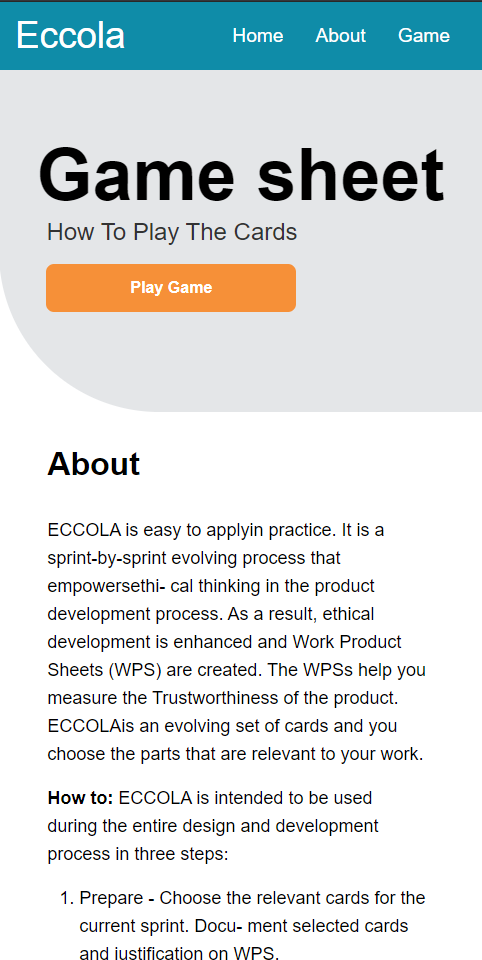
\includegraphics[width=0.5\textwidth]{img/eccola_celular.png}
    \caption{Imagem do sistema adaptado para telas de \textit{smartphones} e \textit{tablets}}
    \label{fig:eccola_celular}
\end{figure}

\begin{figure}[h!]
    \centering
    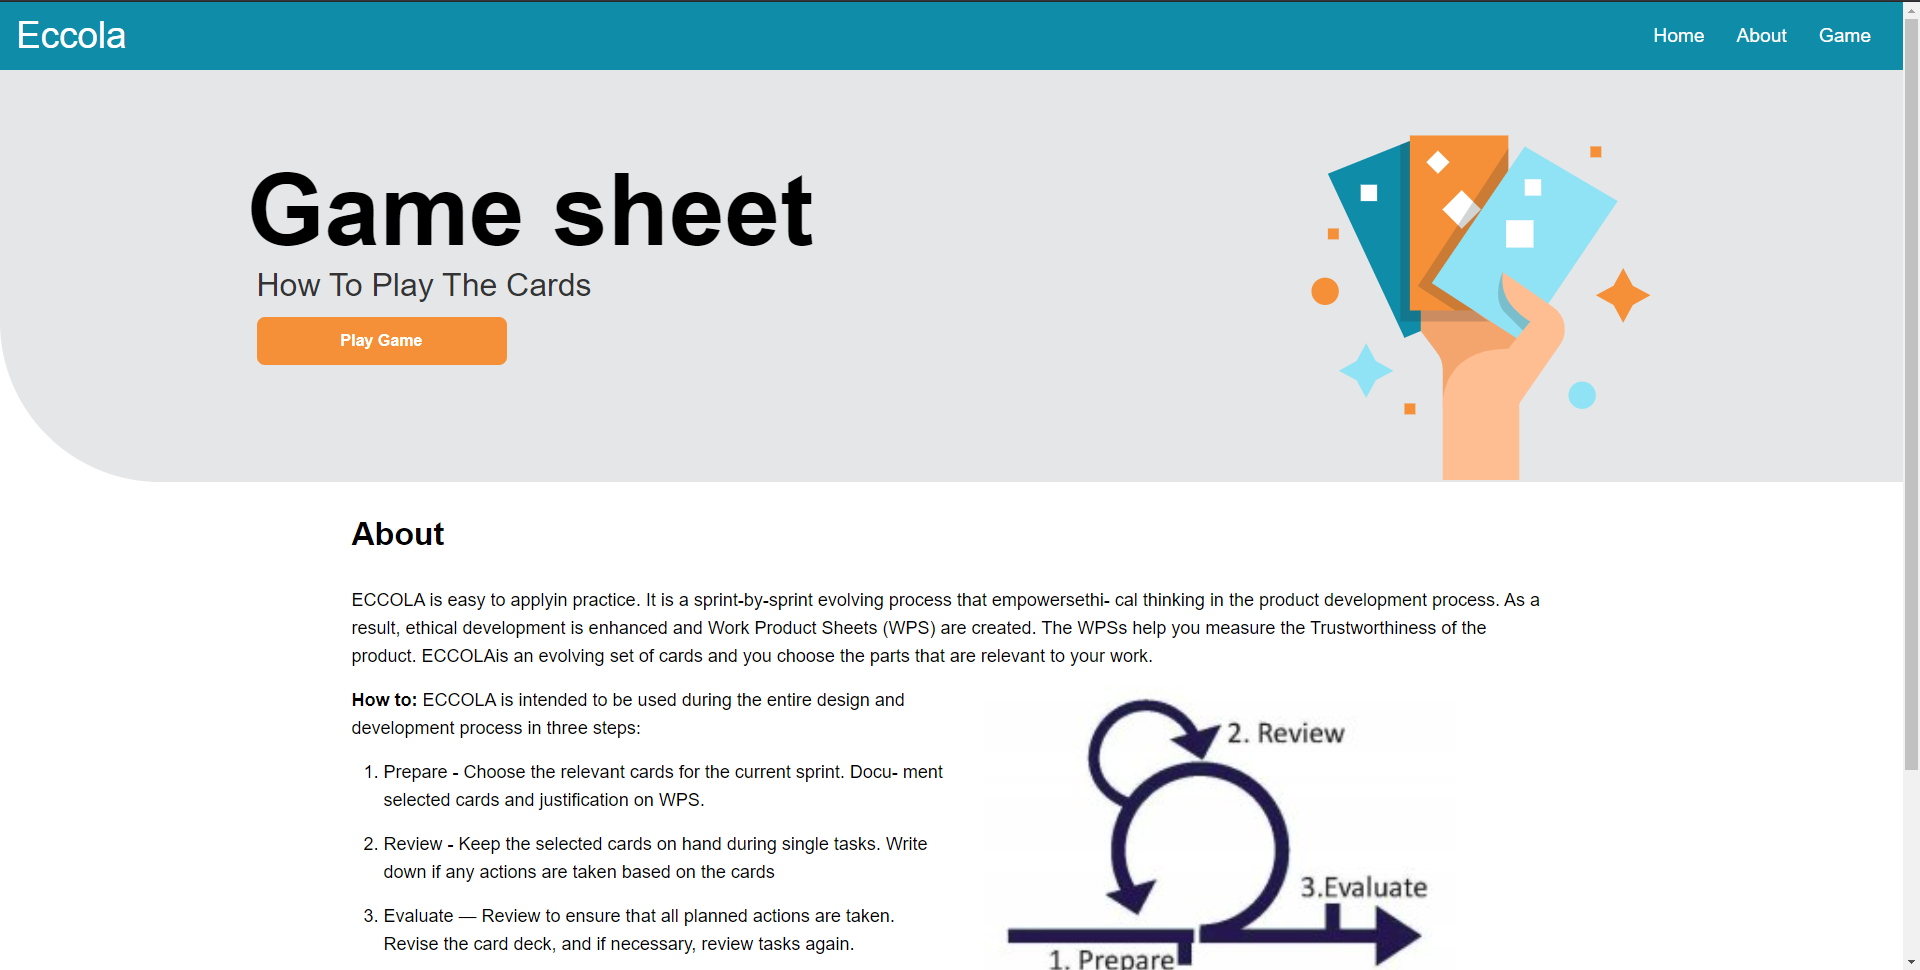
\includegraphics[width=\textwidth]{img/eccola_desktop.png}
    \caption{Imagem do sistema adaptado para telas de computadores de mesa e \textit{notebooks}.}
    \label{fig:eccola_desktop}
\end{figure}

\subsection{Interface}

Para a criação deste guia, a partir da inspiração de um \textit{Planning Poker} voltado para o debate de projetos, foi inspirado que o sistema deveria apresentar seus tópicos através do formato de cards. Para tanto, vendo como o ECCOLA \cite{ECCOLA} fez a implantação em forma analógica (\textit{cards} físicos) do modelo e o mesmo pode ser aplicado para qualquer outro conjunto de regras de elicitação de requisitos de ética em \acrshort{IA}, foi julgado que adotar o modelo de cartas para a criação deste guia seria ainda o ideal.

Para tanto, usamos a plataforma de desenvolvimento de protótipos \href{https://www.figma.com/}{FIGMA}, no qual foi possível desenhar como seria o formato do guia e, a partir dele, criar um \textit{mockup} do que viria a ser o guia. Após a realização de um \textit{brainstorm} sobre como desenvolver o projeto, foi entendido que era necessário que o sistema apresentasse ao menos três telas, sendo uma de boas vindas do sistema, apresentando as regras do jogo, o que é e o título do sistema, uma com os \textit{cards} a serem mostrados aos participantes do planejamento e a tela onde se apresentam as cartas selecionadas apenas, com a opção de retorno e selecionar novamente as cartas. Ao término do projeto de prototipação, chegamos no desenho atual do guia, que pode ser acessado clicando \href{https://www.figma.com/file/zW8ISzBYMcIZFk6BoXZD4n/Eccola}{aqui}.

Com fortes inspirações nos modelos utilizados pelo design gráfico criado pelo Google, o Material Design influenciou fortemente na criação da interface dos \textit{cards}, ajudando-nos a adotar um modelo de \textit{card} que pudesse ser facilmente replicado e identificado, sem perder a característica de um visual limpo, informativo e agradável visualmente, independente da plataforma ao qual o guia esteja sendo utilizado. 

\begin{figure}[h!]
    \centering
    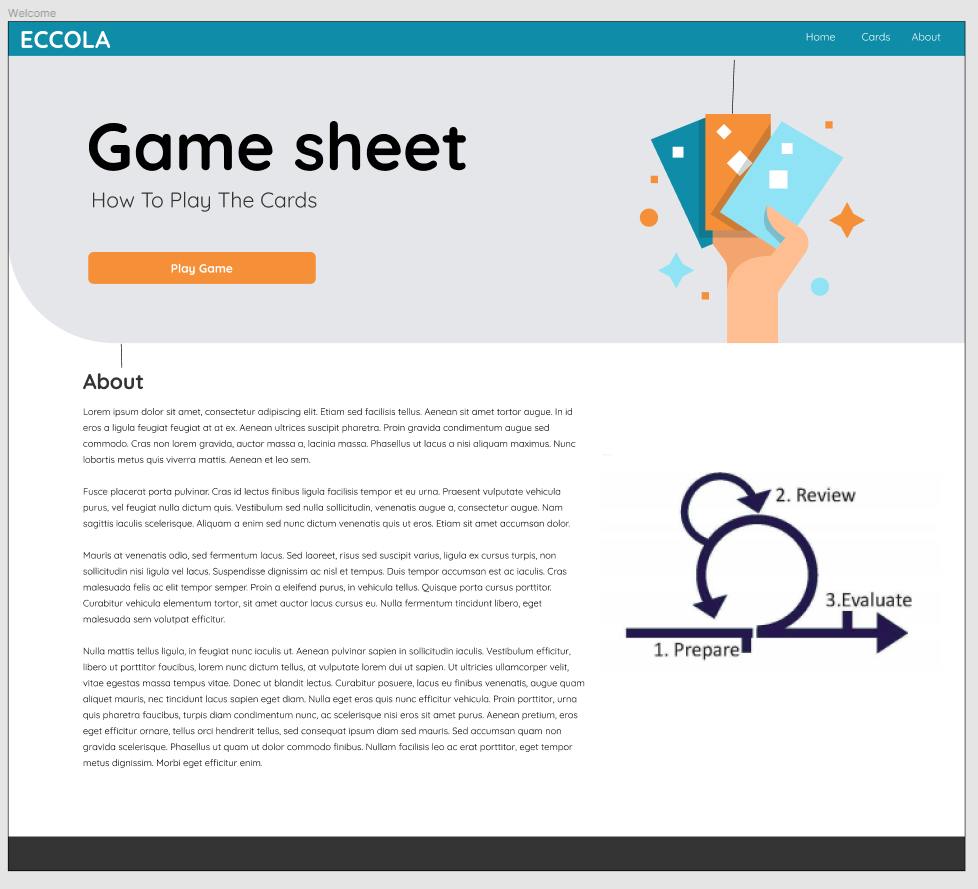
\includegraphics[width=\textwidth]{img/figma_welcome.png}
    \caption{Imagem do protótipo do sistema na tela inicial criado na ferramenta Figma.}
    \label{fig:figma_welcome}
\end{figure}

Para a tela de boas vindas, um design com poucas distrações, uma descrição de como se utilizar o sistema e a possibilidade de se inserir um arquivo mostrando como se trabalhar com as cartas (uma vez que estas são pensadas para serem utilizadas em projetos variados de elicitação de requisitos) ou outras descrições. Para tanto, basta que um usuário com conhecimentos em HTML altere a página inicial ao seu gosto, de acordo as necessidades criadas pelo projeto a ser utilizado junto ao guia.

\begin{figure}[h!]
    \centering
    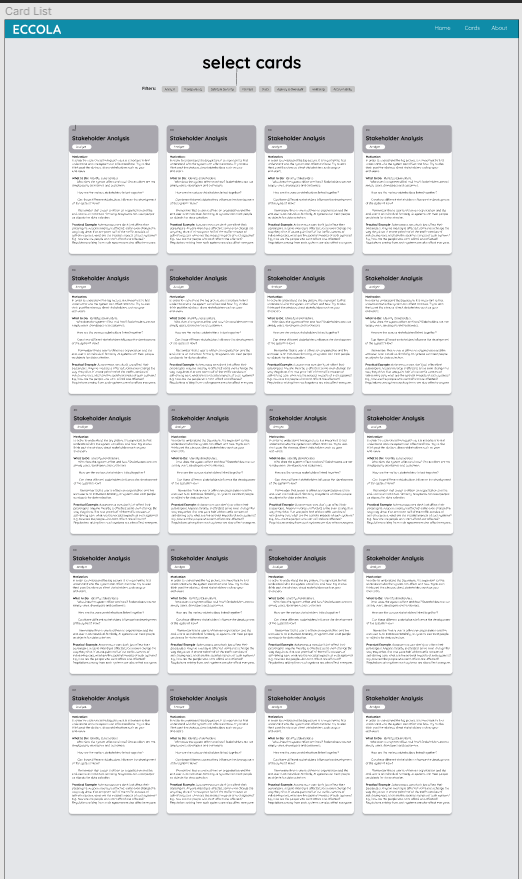
\includegraphics[width=0.7\textwidth]{img/figma_cards.png}
    \caption{Imagem do protótipo do sistema na tela de seleção de \textit{cards} criado na ferramenta Figma.}
    \label{fig:figma_cards}
\end{figure}

Para a tela de escolha dos cards, temos todos os \textit{cards} apresentados, com um menu \textit{drop-down} para o filtro de seleção da categoria das cartas a serem escolhidas para a rodada de debate. Estas cartas e suas categorizações serão melhor detalhadas na seção \ref{Utilizando os cards}. Temos também o botão \textit{Compare cards}, onde após a seleção dos itens para o debate teremos o prosseguimento para a tela de resultados após apertar no botão.

\begin{figure}[h!]
    \centering
    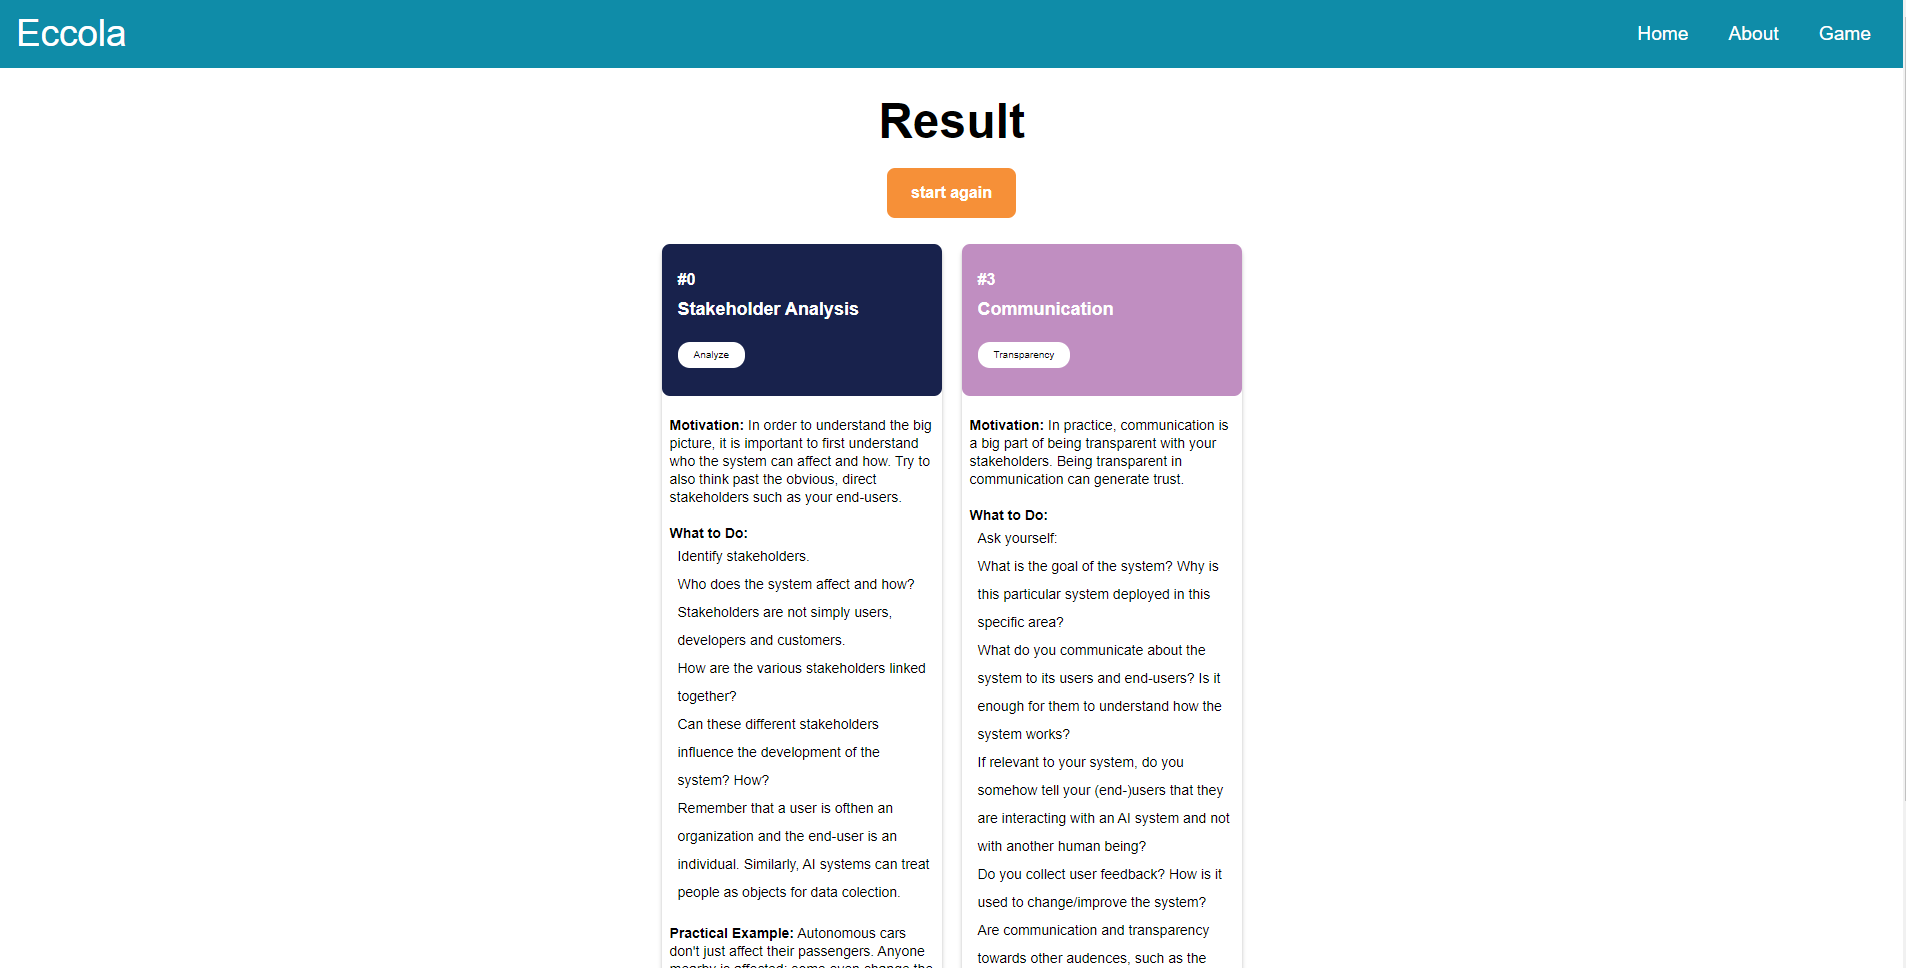
\includegraphics[width=\textwidth]{img/eccola_results.png}
    \caption{Imagem do sistema na tela de \textit{cards} selecionados.}
    \label{fig:eccola_results}
\end{figure}

Para a tela de resultados, durante a prototipação foi deixada a tela propositalmente em branco, porém na versão atual do sistema temos a apresentação das cartas selecionadas na tela anterior juntamente com o botão \textit{Start again}, que permite, caso queira, realizar uma nova seleção dos itens para o debate, o que será abordado em maiores detalhes na Seção \ref{Como utilizar}.

\section{Como utilizar}
\label{Como utilizar}

Tomando como referência o ECCOLA, apresentado na Figura \ref{fig:eccola_desktop}, o sistema terá a tela inicial apresentando tanto um botão ``Play game'', seja no topo da tela ou ao final (inclusive no modo para dispositivos móveis) e os links Home, About e Game no topo da tela, onde cada um dos links envia para uma das páginas (as quais podem ser customizadas e serão detalhadas em maior profundidade na Seção \ref{editandocards}) citadas. Neste caso, o link \textit{Home} encaminha para a página inicial, o link \textit{About} para o espaço onde está a descrição do jogo a ser inserida e o link \textit{Game} para a página onde se encontram as cartas. O botão \textit{Play the Game} localizadas tanto no início quanto final da página  tem o mesmo propósito do link \textit{Game}, levando também para a página onde o \textit{Planning Poker} será realizado.

Na interface do \textit{Planning Poker}, como mostrado na figura \ref{fig:eccola_cards}, temos um menu \textit{dropdown} que serve como filtro, onde somente as cartas do tipo selecionado estarão sendo exibidas na tela caso o filtro \textit{ALL} não esteja ativo, o botão \textit{Compare Cards}, que será acionado somente em caso de selecionar dois \textit{cards} para a discussão (onde o número de \textit{cards} também pode ser alterado, como veremos adiante) e logo abaixo os \textit{cards} que estarão disponíveis para a seleção e discussão. Ao clicar em cada um dos cards, eles terão uma borda laranja ao selecionar os mesmos, onde após clicar no botão \textit{Compare Cards} teremos a tela mostrando apenas os \textit{cards} selecionados. Estes serão os \textit{cards} a serem utilizados no debate, e será apresentado como utilizá-los na Seção \ref{utilizandocards}.

\begin{figure}[h!]
    \centering
    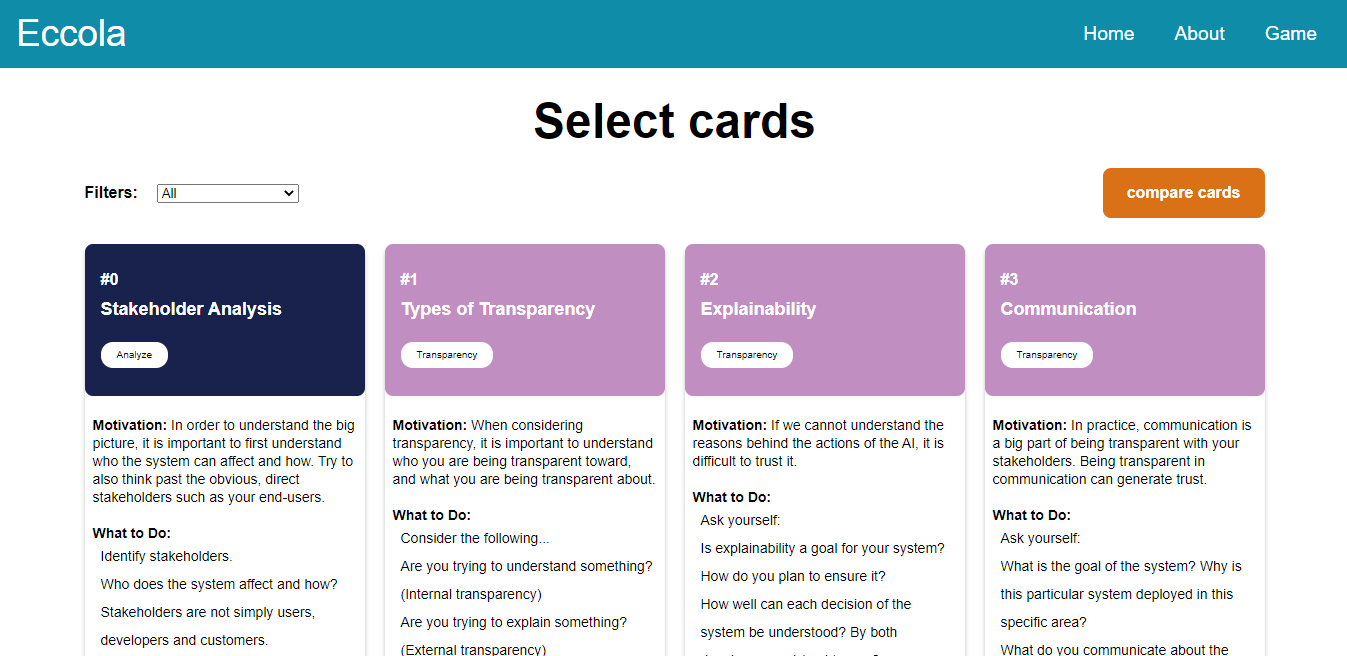
\includegraphics[width=\textwidth]{img/eccola_cards.png}
    \caption{Imagem do sistema com os \textit{cards} disponíveis em uma tela com resolução maior que 640 pixels.}
    \label{fig:eccola_cards}
\end{figure}

\subsection{Utilizando os \textit{cards}}
\label{utilizandocards}
Para a utilização do sistema, é necessário retomarmos aos conceitos de um \textit{Planning Poker} e adaptarmos ao uso no contexto de ética em IA. Para um melhor entendimento, temos que também adaptar o debate ao ambiente de desenvolvimento ágil e o uso do Scrum, já que sem estas ferramentas o uso deste guia fica muito mais limitado.

Para tanto, repensando o contexto de planejamento de um projeto, temos que ter desde o princípio do projeto que o mesmo funcionará através de iterações contínuas e constantes, as quais devem sempre estarem contextualizadas durante o progresso de seu serviço, porém também dando a liberdade ao usuário adaptar a ferramenta de acordo o contexto ao qual se encontra no devido momento.

Desta forma, este guia tem como função balizar os desenvolvedores e \textit{stakeholders} a terem um melhor entendimento de como aplicar os princípios éticos da \acrshort{IA} ao projeto o qual está sendo implantado, uma vez que apesar de se ter a implantação técnica de um lado, através de como será desenvolvido o algoritmo e em qual linguagem, temos também na abordagem do assunto ético diretrizes que vão guiar o comportamento futuro da aplicação perante o ambiente ao qual esta estará inserida e em pleno funcionamento. 

Portanto, acima de tudo, o uso dos \textit{cards} vão servir para que os desenvolvedores possam entender, avaliar, mensurar e revisar a extensão que sua aplicação possa vir a apresentar durante seu ciclo de vida, permitindo assim que este guia seja uma ferramenta que se encaixa plenamente no conceito de desenvolvimento ágil junto com as ferramentas pré-existentes.

No sistema, teremos os \textit{cards} dispostos de acordo o seu proponente apresentar para a equipe. Para fins de conceito, estaremos utilizando os \textit{cards} descritos no sistema ECCOLA \cite{ECCOLA}, uma vez que estes se baseiam nos princípios citados por Ryan e Stahl \cite{Ryan2020ArtificialIE}.

Para o uso dos \textit{cards} em si, independente das regras pré-definidas, é necessário que sempre haja pelo menos dois \textit{cards} escolhidos para o debate. Verifica-se esta necessidade por, segundo Ryan e Stahl \cite{Ryan2020ArtificialIE} termos onze princípios que balizam, praticamente, todos os pontos de debate que veremos em qualquer outro guia a ser montado com auxílio desta ferramenta. E não obstante, o enriquecimento da discussão durante o desenvolvimento da parte técnica da ferramenta pode ser aprimorado com o uso adequado de mais de um \textit{card}, uma vez que haverão pontos de discussão que irão cruzar entre si e delimitar em um ponto que ajudará a apontar se o desenvolvimento da ferramenta em debate está adequado para o contexto em que se encontra, podendo assim criar uma folha de trabalho do produto.

Uma vez selecionados e a discussão aberta, se faz a revisão dos princípios a cada \textit{card} e tema percorrido, visando, assim como no modelo de desenvolvimento Scrum e o andamento de uma \textit{sprint} (preferencialmente durante a discussão dos épicos e histórias, sempre preparar o ambiente com uma visão inicial e um apontamento pré-definido, a revisão do caminho tomado, já que ajustes e correções são necessárias ao longo da implantação do projeto, assim como na parte de implantação do código, para assim se chegar na fase final de avaliação, e verificar se os pontos foram devidamente atendidos.

Durante cada um destes processos, escrever a parte um guia, este qual ajudará na fase de retrospectiva da \textit{sprint}, servindo de guia no que foi trabalho, no que não foi e servindo de aprimoramento para a próxima. 

Com isso, podemos resumir os pontos debatidos acima em três:
\begin{enumerate}
    \item Preparar: Escolher os \textit{cards} para a \textit{sprint} corrente , documentar e justificar suas escolhas em uma folha de trabalho do produto. 
    \item Revisar: Manter os \textit{cards} selecionados à vista durante as tarefas e escrever se alguma ação foi tomada baseada nos \textit{cards}.
    \item Avaliar: Revisar o trabalho feito para garantir que as ações planejadas foram tomadas. Revisar os \textit{cards}, e se necessário, revisar as tarefas novamente.
\end{enumerate}

Como observado pelo Vakkuri et al. \cite{ECCOLA}, é recomendado que a cada sprint estes processos sejam repetidos em todas as iterações, e chegando ao final da sprint que seja realizado uma retrospectiva, discutindo no que foi trabalhado, no que não foi trabalhado e quais as partes são relevantes para a próxima sprint do desenvolvimento do produto.



\section{Documentação}
Temos nesta seção a descrição do sistema feito como um \textit{webapp}, mostrando trechos do código e como ele se encontra em cada um dos arquivos. De uma forma geral, temos no arquivo \textbf{index.html} a página inicial do guia, contendo a tela inicial e uma pequena instrução de como se utilizar o sistema, o arquivo \textbf{game.html} contendo a página que receberá os \textit{cards} do sistema, os arquivos .css \textit{game}, que apresenta a estilização dos \textit{cards}, \textit{style}, responsável pelos aspectos gráficos dos HTML e \textit{reset}, a função que ajuda a jogar novamente o \textit{Planning Poker} sem necessitar recarregar a página para tal. Estaremos a seguir descrevendo cada um dos arquivos com maiores detalhes, demonstrando algumas de seus detalhes técnicos na produção deste sistema e como cada módulo foi pensado para a criação, manutenção e atualização futura.

\subsection{\textit{index.html}}
\begin{lstlisting}[language=HTML, caption=JavaScript example]{
    <nav class="nav">
        <a  href="index.html" class="nav__logo">Eccola</a>
        <ul class="menu">
          <li class="menu__item"><a href="index.html">Home</a></li>
          <li class="menu__item"><a href="#about">About</a></li>
          <li class="menu__item"><a href="game.html">Game</a></li>
        </ul>
    </nav>
};
\end{lstlisting}

\subsection{\textit{game.html}}
Falar sobre a 

\subsection{\textit{game}, \textit{style} e \textit{reset.css}}
Falar sobre a estilização do sistema com o uso de .css

\subsection{\textit{index.js}}
Falar sobre o motor do sistema

\subsection{\textit{infosCards.js}}
Falar sobre o módulo que facilita a criação das cartas.


%%%
Descrever um pouco da documentação, do processo de escrita do framework e apresentar trechos do código que podem ser pertinentes para seu devido entendimento. Explicar o contexto de código autodocumentável, como ele foi aplicado neste trabalho e como ele pode ajudar em trabalhos futuros se mantido o padrão de criação do código. Descrever os principais campos dos arquivos .js e .html, já que o .css foi explicado. Relacionar o game.html, .css, index.js e infosCards.js e como estes quatro componentes se complementam.

\section{Editando os \textit{cards}}
\label{editandocards}

%Parei aqui a leitura 
\begin{itemize}
    \item Explicar cada campo da carta no arquivo infosCards.js
    \item Como editar uma carta
    \item Como inserir uma nova carta para classe já existente
    \item Como inserir uma nova classe para uma nova carta
     \item Explicar como editar o .css para criar a nova carta
    \item Explicar a inserção da carta editando os arquivos game.html, index.js e infosCards.js
\end{itemize}

Além da inserção de parte do código-fonte de como as cartas foram estruturadas, o que cada campo pode fazer e como cada campo pode ser alterado após criar um \textit{fork} -- uma cópia -- do repositório no GitHub para adequação de guias futuros a serem desenvolvidos por quem se interessar.
\todo[inline]{Inserir snippet codigo de carta}


\begin{lstlisting}[language=JavaScript, caption=JavaScript example]
const statePageResult = () => {
  buttonResult.style.display = "none";
  filterContainer.style.display = "none";

  startAgain.style.display = "block"
  container.style.display = "flex";
  container.style.justifyContent="center";

  titlePage.innerText = "Result";
  alert.style.display = "none";
};
\end{lstlisting}


\section{Síntese do Capítulo}